\documentclass[12pt]{article}
\usepackage{geometry}
\usepackage{blindtext}
\usepackage{changepage}
\usepackage{indentfirst}
\usepackage{float}
\parindent=0pt
\usepackage{graphicx}
\graphicspath{ {C:/Users/Eddie/Documents/heart_disease_project/}}
\geometry{left=1in, top=1in, right=1in}
\usepackage[activate={true,nocompatibility},final,tracking=true,kerning=true,factor=1100,stretch=10,shrink=10]{microtype}
\usepackage[colorlinks=true]{hyperref}
\hypersetup{
linkcolor = black,
urlcolor = blue
}
\title{Logistic Regression on the Presence of Heart Disease}
\author{Edward Yu}
\date{February 09, 2018}
\begin{document}
\maketitle
\tableofcontents

\abstract
This project will create a logistic model regressing potential risk factors of heart disease to predict whether an individual has the presence or absence of heart disease. The results of this project can be used in a few ways: 

\begin{enumerate}
  \item To investigate which risk factors are under more or less important in determining an individual's heart condition. 
  \item This model can be built into pre-screening applications in which users can test for their risk of heart disease, supplementing an individual's regiment of physician check-ups and overall  health and body consciousness.
  \item Aid physicians more mathematically and precisely define risk percentages for their patients, particularly for patients who have mixed heart condition signals. 
  \end{enumerate}
\pagebreak
\section{Growing Problem of Heart Disease}
Heart and cardiovascular disease is the leading cause of death worldwide, accounting for approximately 17.3 million deaths per year, and the pangs of this disease are only expected to worsen. By 2030, that number is expected to grow to more than 23.6 million. This accounts for nearly one out of every three deaths. To put a dollar sign to this problem, direct and indirect costs of cardiovascular diseases add up to more than \$320.1 billion in the U.S. in medical costs and lost productivity\footnote{\href{https://healthmetrics.heart.org/wp-content/uploads/2017/06/Heart-Disease-and-Stroke-Statistics-2017-ucm_491265.pdf}{Heart Disease Stats}}.

  As we explore more about the risk factors of heart disease and find innovative ways to detect its presence, we can begin to make smarter decisions about our health. 

\section{Data Set Variables and Descriptions}
This project uses the UCI machine learning repository's \href{http://archive.ics.uci.edu/ml/datasets/Heart+Disease}{Heart Disease Data Set}. The directory contains 4 databases concerning heart disease diagnosis from 4 locations: 

\begin{itemize} 
  \item Cleveland Clinic Foundation (cleveland.data)
  \item Hungarian Institute of Cardiology, Budapest (hungarian.data)
  \item V.A. Medical Center, Long Beach, CA (long-beach-va.data)
 \item University Hospital, Zurich, Switzerland (switzerland.data)
\end{itemize}
Each database contained the same data formatting with a total of 14 attributes. Below are the data variables and descriptions: 
  \begin{adjustwidth}{-1cm}{}
\begin{tabular}{ |p{2cm}|p{13.5cm}| }
\hline
Variable & Definition\\
\hline
age & Age in Years \\
\hline
sex & Sex of Patient (1:male; 0:female)\\
\hline
cp & Chest pain type (1=typical angina; 2=atypical angina; 3=non-anginal pain; 4=asyomptomatic)\\
\hline
trestbps & Resting blood pressure in mm Hg\\
\hline
chol & Serum cholestoral in mg/dl \\
\hline
fbs & Fasting Blood sugar 120 mg/dl (1=true; 0=false)\\
\hline
restecg & Resting electrocardiographic results (0=normal; 1=having ST-T wave abnormality; 2= showing probable or definite left ventricular hypertrophy by Estes' criteria\\
\hline
thalach & Maximum heart rate achieved\\
\hline
exang & Exercise induced angina (1=yes; 2=no)\\
\hline
oldpeak & ST depression induced by exercise relative to rest\\ 
\hline
slope & Slope of the peak exercise ST segment (1=upsloping; 2=flat; 3=downsloping)\\ 
\hline
ca & Number of major vessels\\
\hline
thal & Thallium heart scan, indicates areas of heart that are not getting adequate supply of blood (3=normal; 6=fixed defect; 7=reversable defect\\
\hline
num & Diagnosis of heart disease angiographic diseases status (0= \textless 50\% diameter narrowing; 1= \textless 50\% diameter narrowing)\\
\hline
\end{tabular}
\end{adjustwidth}

\section{Data Wrangling}

Since the data spread across 4 locations contained the same variable structure, the primary goal was to append the rows of each data set into one master data set. Because each observation in the four data sets represented a unique, independent observation the data was already in TIDY structure. Before appending the data observations together variables within each data set was changed to the same variable type. The most important step of this process was converting numerically coded values into proper factors. For example, variable 'cp', chest pain type, was originally coded with a numeric value from 1-4, each associated with a type of chest pain. These values were recoded to character variables describing the chest pain and then factorized. 

The dependent variable 'num' is an integer valued from presence (values 1-4) from 0 (no presence). Because we are simply attemping to distinguish from a set of features whether or not a patient has the presence of heart disease, values \textgreater 0 were coded as 1, thus creating two levels "Presence" and "Absence". From this step, the dependent variable is primed for logistic regression techniques. 

A new variable called 'dsetid' was created denoting which data set each observation came from. This was used to detect any non-random missing value distributions from data set to data set. This variable will not be used in the actual modeling and analysis sections.

Lastly, after variables from each data set were coerced to uniform variable types, each regional data set was row binded together and 'heartDT' became the resulting final data set ready for exploratory analysis.


\section{Exploratory Analysis}
The initial heart data set contains a total of 916 observations and 15 variables. Below is a breakdown of each variable, class, and type: 

\begin{center}
\begin{tabular}{|p{2cm}|p{2cm}|p{2cm}|}

\hline
Variables & Class & Type\\
\hline
age & Numerical & Continuous\\
\hline
sex & Factor & Categorical\\
\hline
cp & Factor & Categorical\\
\hline
trestbps & Numerical & Continous\\
\hline
chol & Numerical & Continuous\\
\hline
fbs & Factor & Categorical\\
\hline
restecg & Factor & Categorical\\
\hline
thalach & Numerical & Continuous\\
\hline
exang & Factor & Categorical\\
\hline
oldpeak & Numerical & Continuous\\
\hline
slope & Factor & Categorical\\
\hline
ca & Factor & Categorical\\
\hline
thal & Factor & Categorical\\
\hline
num & Factor & Categorical\\
\hline
\end{tabular}
\end{center}


\subsection{Dealing with Missing Values: Making the Cut}
A total of 12.74\% of the data was missing. Below is a visual graph of the missingness of each variable, we see the following breakout: 
\begin{center}
\begin{figure}[h!]
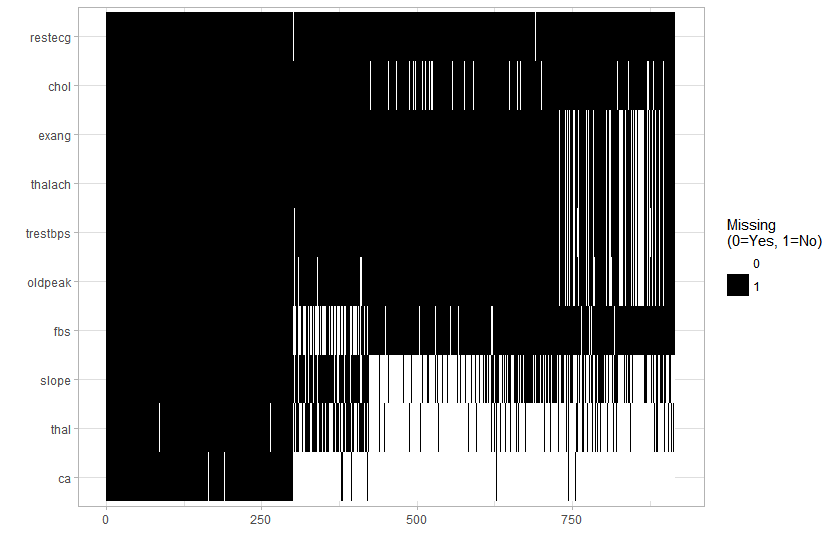
\includegraphics[width=\linewidth]{PredataMissing}
\caption{Missing Observations by Variable}
\end{figure}
\end{center}
The figure above is sorted in increasing number of missing observations from top to bottom with restecg having the least number of missing variables and ca having the greatest. Variables with no missing values were ommitted from the figure. The variables restcg, chol, exang, thalach, trestbps, oldpeak, and fbs seem to be missing at random. Although it is impossible to verify statistically, it is substantively reasonable to claim these variables do not have any signficant patterns of missingness. Some argument can be made that the variables exang, thalach, trestbps, and old peak have similar lines appearing for the same observations because of the straight white lines that cross through all three variables. These observations are most likely the result of nonresponse from the same individual patients. However, because these observations constitute only a minute percentage of the whole data set the missingness will not affect future analysis significantly and wil be dealt with by imputation. 

  Variables slope, thal, and ca have 33.62\%, 66.37\%, and 52.72\% missingness respectively, which is significantly larger than other variables as denoted by the large white chunks in Figure 1. Because of the particular method of binding rows used: 
  
  \[heartdata <-bind\_rows(cleveland,switzerland,hungarian,longbeach)\]

We know that the first observations within the heartdata set come from the cleveland data set with 302 observations. The observations of switzerland, hungarian, and long beach data sets follow thereafter. This indicates that the majority of missingness from slope, thal, and ca are likely to be from the data set regions of switzerland, hungarian, and long beach. This is further confirmed in the table below: 
\begin{center}
\begin{tabular}{|p{3.5cm}|p{1.5cm}|p{1.5cm}|p{1.5cm}|}
\hline
\multicolumn{4}{|c|}{Missing Variable}\\
\hline
Data Set Region & slope & ca & thal\\
\hline
Cleveland & 0.0\% & 0.4\% & .2\%\\
Switzerland & 1.8\% & 12.7\% & 5.5\%\\
Hungarian & 20.6\% & 31.7\% & 28.9\%\\
Long Beach & 11.1\% & 21.5\% & 18.0\%\\
\hline
\end{tabular}
\end{center}

From the table above, we can conclude that there is a systemic presence of missingness due to regional data collection. Since slope, thal, and ca have a signficant percentage of data missing and is systemic, these variables have been removed from the data set and will be left out in further analysis. Although it may be alluring to impute these variables, the amount of missing data is not trivial and if done so will bias the analysis. 
\pagebreak
\subsection{Imputation of Continuous and Categorical Missing Values}
Missing values for the remaining variables were split into numerical and categorical classifications. Numerical variables were imputed using the predicted mean method. Categorical variables were imputed using Bayesian polytomous regression since the factored are unordered and contain more than two levels. 

The distribution of original and imputed numeric data is displayed in the density graph below: 

\begin{figure}[h!]
\begin{center}
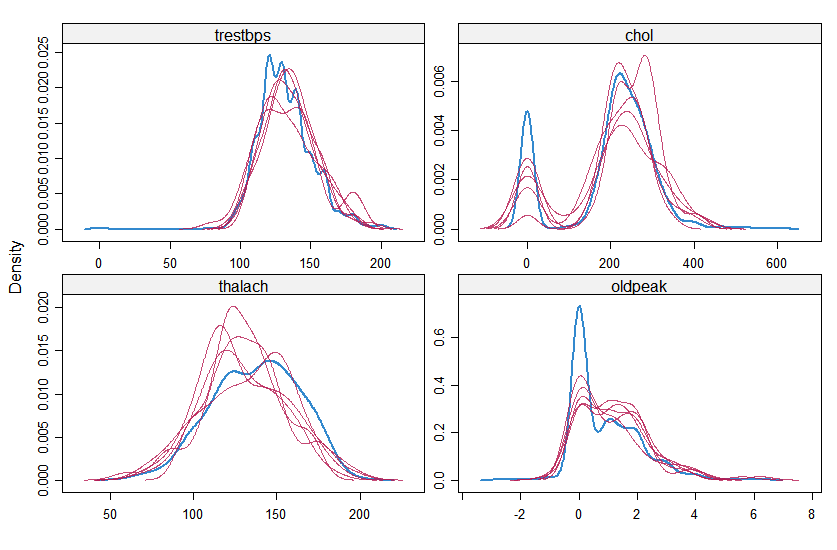
\includegraphics[scale=.35]{density_impute_num}
\caption{Density graph of imputed numeric data}
\end{center}
\end{figure}
The blue lines represent the density of the original data while the magenta line represents the imputed data distribution. We see that trestbps and chol have very similar lines densities. Thalach's imputed distribution shows a higher peak distribution in the low 100's as compared to the original data. Oldpeak original has a higher density centered around 0. For the most part the matching shape of the blue and magenta lines indicate that the imputed values are plausible values with similar distributions as the original data. Another graph, the strip plot, shares a similar story:

\begin{figure}[h!]
\begin{center}
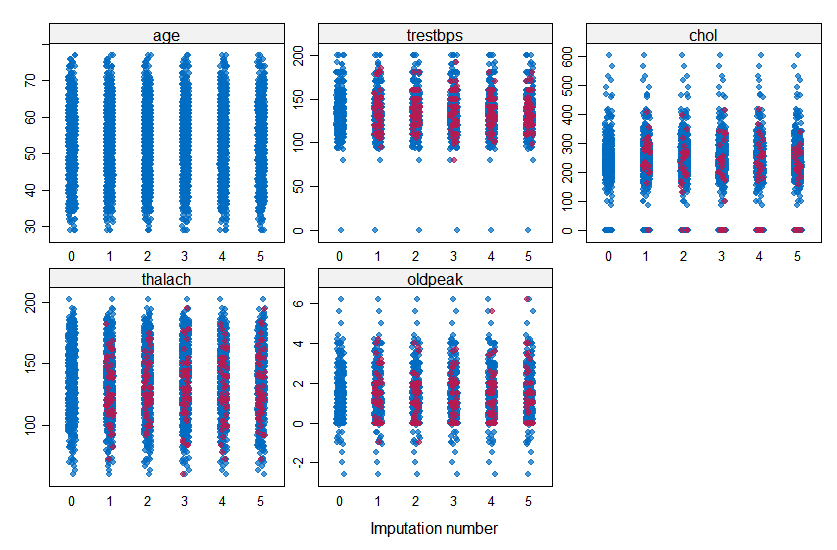
\includegraphics[scale=.35]{strip_impute_num}
\caption{Density graph of imputed numeric data}
\end{center}
\end{figure}
Age is also displayed within the strip plot, but because age did not contain any missing observations all dots were blue. 

A strip plot of categorical data imputation was also created: 
\begin{figure}[h!]
\begin{center}
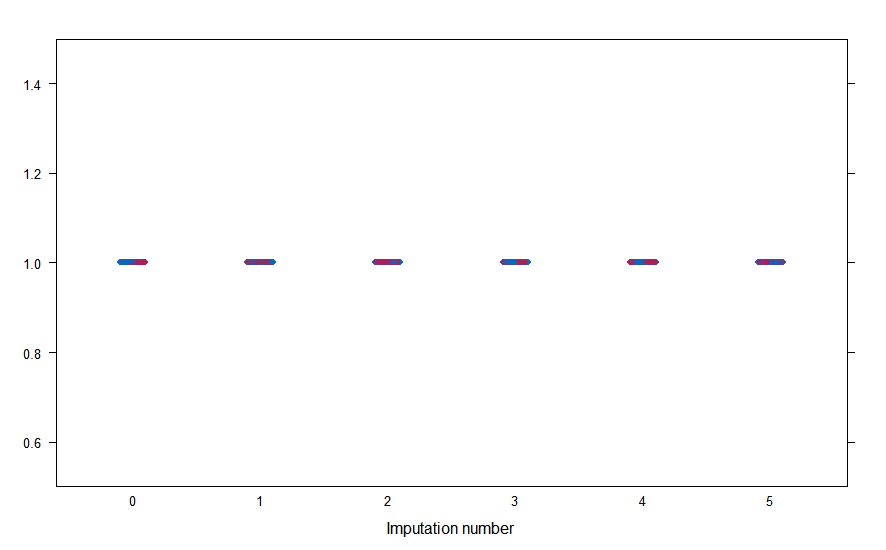
\includegraphics[scale=.35]{strip_impute_cat}
\caption{Density graph of imputed numeric data}
\end{center}
\end{figure}

Blue and magenta dots overlap on each other indicating the imputed values are close to the real values. Both numeric and categorical imputed values replaced the original missing values within the 'heartDT' set, thus finalizing the 'heartDT' data set for model selection and logistic regression analysis. 

\subsection{Correlation Plots}
Numerical variables were separated from categorical variables from the 'heartDT' data set. The corrplot function was used to create the following correlation plot: 

\begin{figure}[h!]
\begin{center}
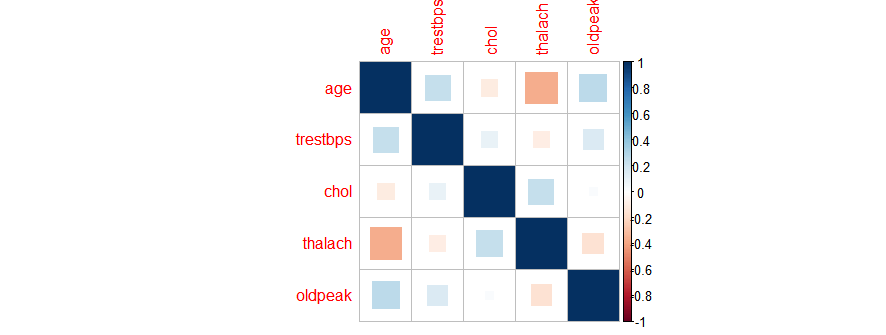
\includegraphics[scale=.75]{correlation}
\caption{Correlation Plot of Numeric Variables}
\end{center}
\end{figure}
From the correlation plot we can see there is no strong correlation between any of the numeric variables. Age did have a weak correlation with trestbps and oldpeak, and chol with thalach had a similar correlation of 0.4. 

\section{Model Selection}
Starting with 916 total observations in the 'heartDT' data set the master data set was split into training and testing data sets. 75\% of the data was allocated to the training and 25\% to the testing. All model selections were trained on the training set and then tested using the testing set. The featured model selection methods tested in this project will be forward stepwise, backward stepwise, and L1 regularization (LASSO). The forward and backwards stepwise's performance will be tested on AIC criteria. The strengths and weaknesses of each model selection method will then be discussed and compared. 

\subsection{LASSO method}
In the world of statistics, LASSO and its related techniques such as Ridge regression and Elastic net are fairly newer methods compared to stepwise regression that have enhanced our ability for prediction accuracy and interpretability of our statistical models. The LASSO method is a way of both variable selection and regularization and offers a parsimonious model by constraining the magnitude of the coefficients, thus making the model simpler and more elegant. 

The 'glmnet' function was used to complete the LASSO regression. After splitting the original 'heartDT', 687 observations was appropriated to the 'heartTrain' data set. The following code was run to fit the first LASSO regression: 

\[fit = glmnet(x=X\_train, y=Y\_train, family = "binomial")\]

where $X\_train$ is a matrix of indepdendent variables and $Y\_train$ is an object containing the 'num' regressed variable. The plot below shows the fit: 

\begin{figure}[h!]
\begin{center}
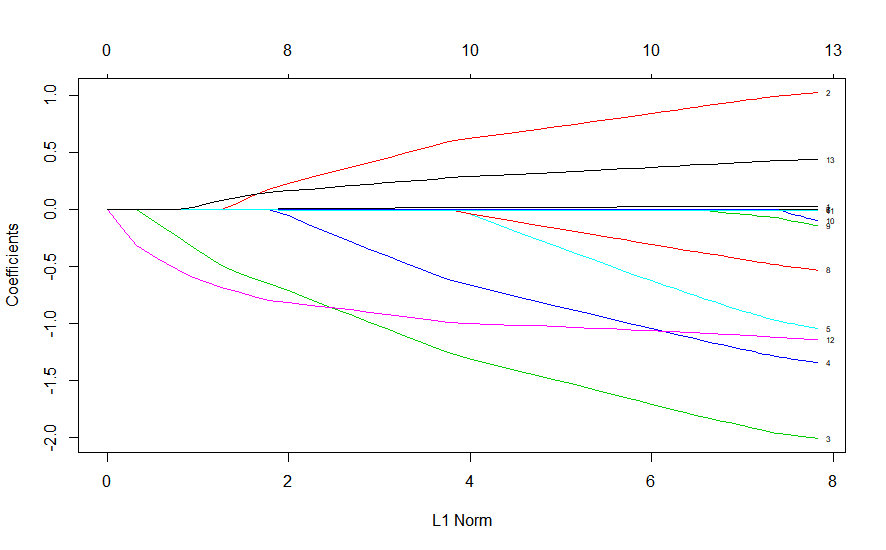
\includegraphics[scale=.5]{fit_l1norm}
\caption{L1 Norm vs. Coefficients from LASSO regression}
\end{center}
\end{figure}

Each curve corresponds to a variable within the model, including each categorical factor with a total of 13 variables. The path of the curve shows its coefficient against the $L_{1}norm$ as $\lambda$ varies. The axis above indicates the number of non-zero coefficients at the current $\lambda$. The $\lambda$ controls trade off between fitting the training data well (minimizing deviance) and keeping the coefficients small. It effectively controls keeping hypothesis relatively simple to avoid overfitting. 
  
When $\lambda$ is small the LASSO regularization term, $L_{1}norm$, the LASSO solution is similar to OLS solution retaining all coefficients. In contrast, a large $\lambda$ value will penalize coefficients highly, increasing the regularization reducing the parameters to zero ending up with an underfit model. Controlling for the $\lambda$ value is essential for managing the complexity of the model. 

\pagebreak
Cross-validation is used to select the most optimal $\lambda$. In choosing a correct value we will consider the end goal of prediction accuracy. The function cv.glmnet conveniently provides us a way of cross-validation:

\[cvfit = cv.glmnet(x=X\_train, y=Y\_train, family = "binomial", type.measure = "class")\]

Below is a graph of the resulting cross-validation error curve:
\begin{figure}[h!]
\begin{center}
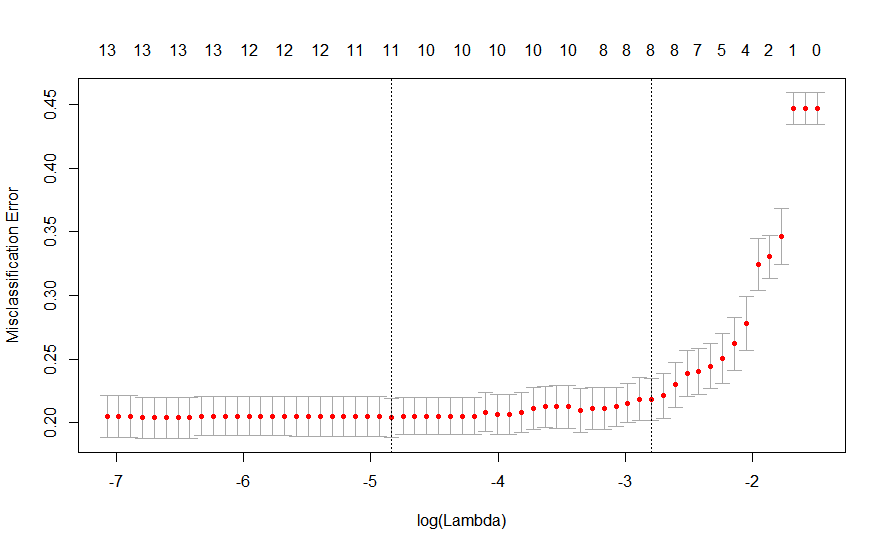
\includegraphics[scale=.5]{cv_error}
\caption{Cross-Validation Curve vs. Lambda}
\end{center}
\end{figure}

The red dotted line represents the cross-validation curve and the error bars represent the the upper and lower standard deviation. A similar trend is seen here with larger $\lambda)$ values leading to an increasing effect of regularization and reducing more coefficients to 0. The two black dotted lines represent the $\lambda)$ value with the minimum CV error and the $\lambda)$ value one standard error away (also representing the slightly more regularized model). We select the $\lambda)$ value with the least CV error because the cross-validation error estimates prediction error, so by choosing the $\lambda)$ with the minimum CV error we are also achieving minimal prediction error. 

Now, we test predictions for both $\lambda_{min}=0.00789$ and $\lambda_{1se}=0.0611$ using the 'heartTest' data set:
\[cv\_pred\_min <-predict(cvfit, newx = X\_test, type = "class", s = cvfit\$lambda.min)\]
\[cv\_pred\_1se <-predict(cvfit, newx = X\_test, type = "class", s = cvfit\$lambda.1se)\]

Analyzing the prediction accuracy with the confusion matrix: 

\begin{figure}[h!]
\begin{center}
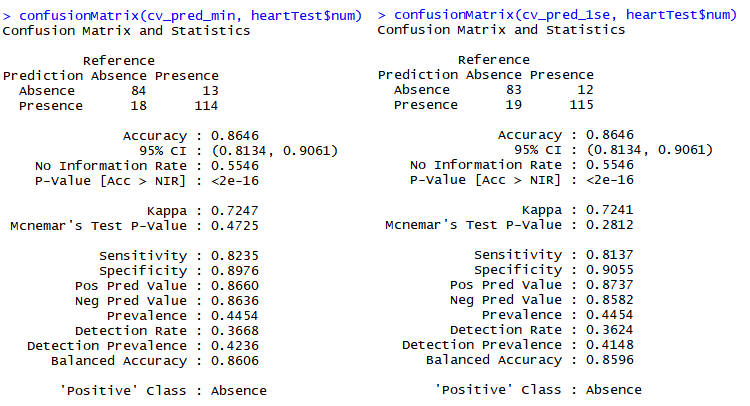
\includegraphics[scale=.75]{confusionmatrix}
\caption{Left: $\lambda_{min}$, Right: $\lambda_{1se}$}
\end{center}
\end{figure}

The accuracy of both models are essentially the same with a small difference of $\lambda_{min}$ having a higher sensitivity and lower specificity than $\lambda_{1se}$. 

\pagebreak
The final features the LASSO model selects are: 
\begin{figure}[h!]
\begin{center}
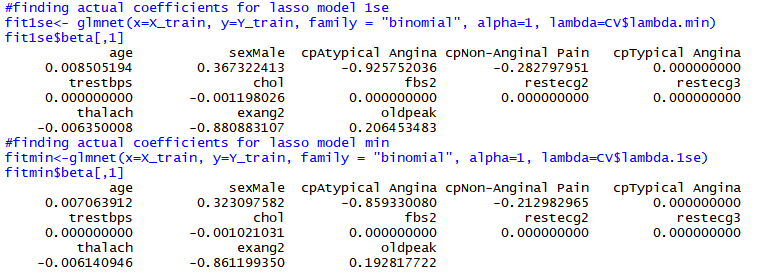
\includegraphics[scale=.75]{lassocoefficients}
\caption{Lasso Model Coefficients; Top:  $\lambda_{1se}$, Bottom: $\lambda_{min}$}
\end{center}
\end{figure}


Plugging in the coefficients into the logistic regression equation we have: 
\[log(\frac{p}{1-p})=\beta_{0}+\beta_{1}*age+\beta_{2}*sexMale+\beta_{3}*cpAtypical Angina+...+\beta_{13}*oldpeak\]

where each $\beta$ is represented by the coefficients listed in Figure 9. In interpreting the model, for example, holding all other variables at a fixed value, the odds of the presence of heart disease if a patient is male rather than female is $e^{0.323}=1.381$. In other words, we can say that the odds for males having heart disease are 38\% higher than the odds for females. 

\pagebreak
\subsection{Forward \& Backwards Stepwise Regression}
The stepwise regression method is an older approach of choosing predictive variables in an automated fashion. Within each step of the process a variable is considered for addition or subtraction from the overall model starting from either a null or full model. The forward model begins by starting with a null model, then slowly steps upwards by adding the most significant model. The backward model begins with the full model and cuts out the least significant model. 

A null model was first created regressing $'num' ~ 1$. Afterwards the 'step' function from the leap package was used to perform the forward stepwise regression. The final model contained the following variables: cp, exang, chol, oldpeak, sex, age, thalach, and fbs. After each step the AIC criteria decreased to a final value of 614.4.

Likewise, a full model containing all variables was first created regressing $'num ~ .$. Afterwards, the 'step' function was used to perform the backward stepwise regression. The final contained the following variables: age, sex, cp, chol, fbs, thalach, exang, and oldpeak. The AIC criteria also was 614.4 for the final model as expected. 
The coefficients for the forwards and backwards stepwise models are shown below: 

For the logistic regression equation we have: 
\[log(\frac{p}{1-p})=\beta_{0}+\beta_{1}*age+\beta_{2}*sexMale+\beta_{3}*cpAtypical Angina+...+\beta_{10}*oldpeak\]

The coefficients for the forwards and backwards stepwise models are shown below: 
\begin{figure}[h!]
\begin{center}
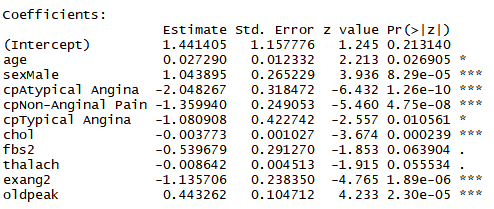
\includegraphics[scale=.75]{coefstepwise}
\caption{Coefficients for Stepwise Models}
\end{center}
\end{figure}

\pagebreak
The confusion model is shown below: 

\begin{figure}[h!]
\begin{center}
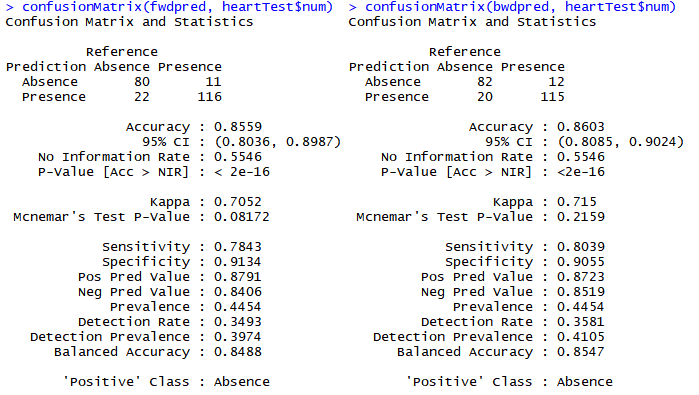
\includegraphics[scale=.75]{confusionmatrix_step}
\caption{Left: Forward Step, Right: Backward Step}
\end{center}
\end{figure}

Both the forward and backward stepwise models produced the same list of variables and had a final AIC value of 614.4. The accuracy of the backwards regression model was slightly higher than the forward model. The sensitivity of the forward model had a lower sensitivity but a greater specitifity. 

\subsection{Model Conclusion}
The primary point of model comparison between LASSO and Stepwise regression methods is prediction accuracy. On testing with 'heartTest' data set, the LASSO method performed slightly better than the Stepwise regression methods. Considering the subset of features within this data set was fairly small with a total of 13 variables, the LASSO regularization method did not have as much of a chance to shine. The LASSO method finds its strength where $p>>n$. $p$, representing the number of features within a model and $n$, representing the number of observations. 
  With a large number of features, the LASSO method does a great job in coercing coefficients to 0, reducing the amount of overfitting. One inherent weakness of L1 regularization is that it tends to do poorly on variable sets with high levels of multicollinearity by often selecting a group of highly correlated variables. However, as we have seen there is not a high level of correlation amongst the numeric variables of this particular data set, thus is not a significant issue here. 

  Overall, regarding the condition of heart disease, the most significant contributor seems to be sexMale having the largest coefficient of 0.323 within the LASSO model. Other indicates such as oldpeak, representing ST depression is often a sign of myocardial ischemia, which is the lack of blood supply to the heart. In a cardiac stress test, a change of at least 2 mm signifies reversible ischemia. Any mm drop greater than 2 from from vertical distance between the patient's trace and isoelectric line is indicative of irreversible ischemia \footnote{\href{http://www.madsci.com/manu/ekg_st-t.htm}{Ischemia Site}}. 
\end{document}      